\documentclass[a4paper, 12pt]{beamer}

\usetheme{CambridgeUS}
\usecolortheme{beaver}
\usefonttheme{structuresmallcapsserif}

%%%%%%%%%% Packages %%%%%%%%%%

\usepackage[slovene]{babel}
\usepackage[utf8]{inputenc}
\usepackage[T1]{fontenc}
\usepackage{lmodern}
\usepackage{units}
\usepackage{eurosym}
\usepackage{amsmath}
\usepackage{amssymb}
\usepackage{amsthm}
\usepackage{amsfonts}
\usepackage{mathtools}
\usepackage{graphicx}
\usepackage{color}
%\usepackage{url}
\usepackage{hyperref}
\usepackage{enumerate}
\usepackage{enumitem}
\usepackage{pifont}
\usepackage[english, croatian, slovene]{babel}

\newcommand{\myitem}{\item[\textbullet]}

\theoremstyle{definition} 
\newtheorem*{definicija}{Definicija}
\newtheorem*{trditev}{Trditev}


\theoremstyle{plain} 
\newtheorem*{izrek}{Izrek}
\newtheorem*{posledica}{Posledica}
\newtheorem*{zgled}{Zgled}
\newtheorem{primer}{Primer}


\definecolor{bostonuniversityred}{rgb}{0.8, 0.0, 0.0}

%%%%%%%%%%%%%%%%%%%%%%%%%%%%%%%%%%%%%%%%%%%%%%%%%%%%%%%%%%%%%%%%%%%%%%%


\title[Seminar 1 -- SPAA 2020]{\textbf{ACM Symposium on Parallel in Algorithms and Architectures}
\\
Conference SPAA 2020
}

\author[FRI, Algoritmi]{Sara Bizjak  \ \ |  \ \ Bor Brecelj  \ \ |  \ \  Zala Erič  \ \ |  \ \  Laura Guzelj Blatnik
\\
\\
}
\institute[]{\small{Fakulteta za računalništvo in informatiko, 
\\
Univerza v Ljubljani}}
\date{Marec 2021}


\begin{document}

\titlepage

%%%%%%%%%%%%%%%%%%%%%%%%%%%%%%%%%%%%%%%%%%%%%%%%%%%%%%%%%%%%%%%%%%%%%%%%%%%%%%%%%%

\begin{frame}
\frametitle{O konferenca SPAA}

    \begin{itemize}
        \item \textbf{Tema:} hkratno izvajanje operacij računalniškega sistema.
        \item \textbf{Nameni in cilji:} 
        \begin{itemize}
            \myitem interes in obiskovanost,
            \myitem poglobiti razumevanje paralelne izračunljivosti.
        \end{itemize}
        \item \textbf{Tematike člankov:} teorija in praksa
        \begin{itemize}
            \myitem paralelni in porazdeljeni algoritmi ter podatkovne strukture,
            \myitem energetsko učinkoviti modeli,
            \myitem upravljanje množičnih podatkovnih nizov,
            \myitem vzporedna teorija zapletenosti,
            \myitem večjedrni sistemi,
            \myitem ...
        \end{itemize}
    \end{itemize}

\end{frame}

%%%%%%%%%%%%%%%%%%%%%%%%%%%%%%%%%%%%%%%%%%%%%%%%%%%%%%%%%%%%%%%%%%%%%%%%%%%%%%%%%%

\begin{frame}
    \frametitle{SPAA 2020}
    
        \begin{itemize}
            \item \textbf{Termin:}
            14. - 16. julij 2020, 32. izvedba, prvič virtualna.
            \item \textbf{Članki:}
            \begin{itemize}
                \myitem prijavljeni: 127,
                \myitem sprejeti: 41 običajnih + 27 prispevkov.
            \end{itemize}
            \item \textbf{Urnik in potek:}
            \begin{itemize}
                \myitem prvi dan: delavnice in vaje,
                \myitem drugi in tretji dan: 12 sej s predstavitvami člankov.
            \end{itemize}
            \item \textbf{Nagrajen članek:} 
            \begin{itemize}
                \item \textit{Sublinear Algorithms in T-interval Dynamic Networks}, 
                \item Irvana Jahja in Haifeng Yuja.
            \end{itemize}
        \end{itemize}
    
    \end{frame}


%%%%%%%%%%%%%%%%%%%%%%%%%%%%%%%%%%%%%%%%%%%%%%%%%%%%%%%%%%%%%%%%%%%%%%%%%%%%%%%%%%
%%%%%%%%%%%%%%%%%%%%%%%%%%%%%%%%%%%%%%%%%%%%%%%%%%%%%%%%%%%%%%%%%%%%%%%%%%%%%%%%%%
%%%%%%%%%%%%%%%%%%%%%%%%%%%%%%%%%%%%%%%%%%%%%%%%%%%%%%%%%%%%%%%%%%%%%%%%%%%%%%%%%%

\section{PRVI IZBRANI ČLANEK}
\begin{frame}
    \frametitle{\small{OPTIMAL PARALLEL ALGORITHMS IN THE BINARY-FORKING MODEL}}
    \begin{itemize}
        \item \textbf{Avtorji:} G.~E.~Blelloch, J.~T.~Fineman, Y.~Gu in Y.~Sun.
        \item \textbf{Opažanje:} vzporedne algoritme ponavadi analiziramo v modelu PRAM.
        \item \textbf{Problem:} model PRAM ni realističen.
        \item \textbf{Rešitev:} optimalni algoritmi za nekaj problemov v binary-forking modelu.
    \end{itemize}
    \begin{figure}[H]
        \centering
        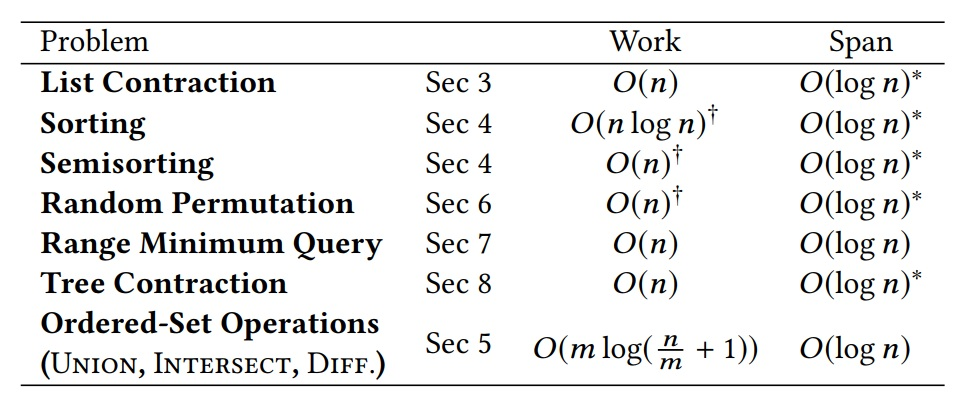
\includegraphics[width=60mm]{binary_forking.jpg}
        \caption{Časovne zahtevnosti predstavljenih algoritmov.}
    \end{figure}

\end{frame}


%%%%%%%%%%%%%%%%%%%%%%%%%%%%%%%%%%%%%%%%%%%%%%%%%%%%%%%%%%%%%%%%%%%%%%%%%%%%%%%%%%

\section{DRUGI IZBRANI ČLANEK}
\begin{frame}
\frametitle{\small{OPTIMAL RESOURCE ALLOCATION FOR ELASTIC AND INELASTIC JOBS}}
    
    \begin{itemize}
        \item \textbf{Avtorji:} B.~Berg, M.~Harchol-Balter, B.~Moseley, W.~Wang in J.~Whitehouse.
        \item \textbf{Problem:} slabo izkoriščeni resursi v podatkovnih centrih.
        \item \textbf{Ideja:} najti optimalno strategijo za dodeljevanje opravil, če jih ločimo na elastična in neelastična.
        \item \textbf{Rešitev:} 
            \begin{itemize}
                \myitem velikost neelastičnih opravil \textit{enaka} kot elastičnih $\Rightarrow$ Neelastična-prvo je optimalna strategija.
                \myitem velikost neelastičnih opravil \textit{večja} kot elastičnih $\Rightarrow$ Neelastična-prvo je boljša strategija
                \myitem velikost elastičnih opravil \textit{večja} kot elastičnih $\Rightarrow$ Elastično-prvo je boljša strategija.
            \end{itemize}
    \end{itemize}

\end{frame}


%%%%%%%%%%%%%%%%%%%%%%%%%%%%%%%%%%%%%%%%%%%%%%%%%%%%%%%%%%%%%%%%%%%%%%%%%%%%%%%%%%

\section{TRETJI IZBRANI ČLANEK}
\begin{frame}
    \frametitle{\small{RANDOMIZED INCREMENTAL CONVEX HULL IS HIGHLY PARALLEL}}
    
    \begin{itemize}
        \item \textbf{Avtorji:} G.~E.~Blelloch, Y.~Gu, J.~Shun in Y.~Sun.
        \item \textbf{Problem:} paralelizacija algoritma za reševanje problema inkrementalne konveksne lupine točk.
        \item \textbf{Ideja:} dva neodvisna robova lahko v množico dodamo istočasno.
        \item \textbf{Rešitev:} predstavljen algoritem za reševanje problema in dokaz, da je algoritem paralelen z globinsko odvisnostjo $\mathcal{O}(\log n)$.
    \end{itemize}
    \begin{figure}[H]
        \centering
        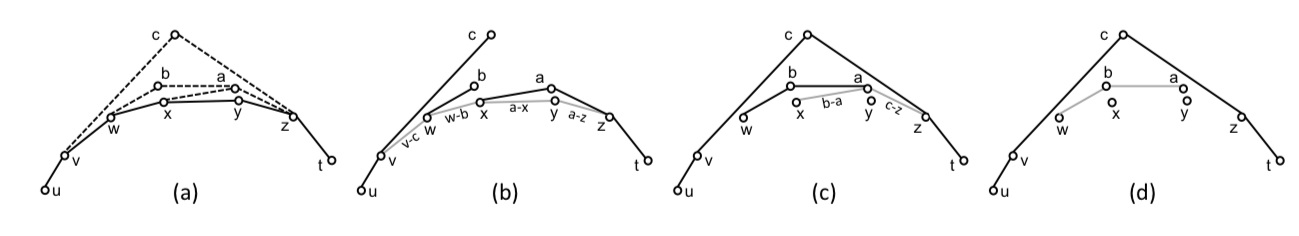
\includegraphics[width=90mm]{convex_hull.jpg}
        \caption{Dodajanje robov pri reševanju problema konveksne lupine.}
    \end{figure}

\end{frame}
    
    
%%%%%%%%%%%%%%%%%%%%%%%%%%%%%%%%%%%%%%%%%%%%%%%%%%%%%%%%%%%%%%%%%%%%%%%%%%%%%%%%%%

%%%%%%%%%%%%%%%%%%%%%%%%%%%%%%%%%%%%%%%%%%%%%%%%%%%%%%%%%%%%%%%%%%%%%%%%%%%%%%%%%%


    
    
%%%%%%%%%%%%%%%%%%%%%%%%%%%%%%%%%%%%%%%%%%%%%%%%%%%%%%%%%%%%%%%%%%%%%%%%%%%%%%%%%%


    
    
%%%%%%%%%%%%%%%%%%%%%%%%%%%%%%%%%%%%%%%%%%%%%%%%%%%%%%%%%%%%%%%%%%%%%%%%%%%%%%%%%%


    
    
%%%%%%%%%%%%%%%%%%%%%%%%%%%%%%%%%%%%%%%%%%%%%%%%%%%%%%%%%%%%%%%%%%%%%%%%%%%%%%%%%%



%%%%%%%%%%%%%%%%%%%%%%%%%%%%%%%%%%%%%%%%%%%%%%%%%%%%%%%%%%%%%%%%%%%%%%%%%%%%%%%%%%


    
    
%%%%%%%%%%%%%%%%%%%%%%%%%%%%%%%%%%%%%%%%%%%%%%%%%%%%%%%%%%%%%%%%%%%%%%%%%%%%%%%%%%



\end{document}
